\subsection{Trasferimento affidabile}
Il trasferimento affidabile è stato realizzato implementando l'algoritmo \emph{selective repeat} descritto nel libro [riferimento].\\
Tale implementazione è stata ``isolata'' all'interno di un modulo apposito, creando un livello di trasporto virtuale,
il quale si occupa di suddividere i messaggi in segmenti di giusta misura e di gestirne gli invii, le ritrasmissioni e la ricezione.

\subsubsection{Interfaccia}
L'interfaccia che offre questo stato di trasporto virtuale, come descritto nei primi capitoli, è simile a quella che un programmatore ha a disposizione per un protocollo TCP.\\
Per richiamare la funzione per l'invio dei dati (\emph{rdt\_send}) basta specificare l'indirizzo e la dimensione del buffer contente i dati da inviare, mentre per la ricezione (\emph{rdt\_recv}) l'indirizzo e la dimensione del buffer che riceverà i dati.\\
A differenza delle comuni \emph{read} e \emph{write} non va specificato il file descriptor della socket, perché il servizio di trasporto virtuale si basa su una connessione, per cui la socket è fissata al momento dell'instaurazione della connessione, che avviene quando viene chiamata la funzione \emph{init\_transport}.\\
Inoltre la funzione \emph{rdt\_read\_string} permette di leggere una stringa di una certa lunghezza massima dal messaggio arrivato, cosa necessaria per poter leggere il nome del file che si vuole scaricare.

\begin{lstlisting}[title=transport.h].
void init_transport(int sockfd, struct proto_params *params);
void rdt_send(const void *buf, size_t len);
void rdt_recv(void *buf, size_t len);
ssize_t rdt_read_string(char *buf, size_t size);
\end{lstlisting}

\subsubsection{Struttura}
Lo strato di trasporto virtuale è visto dall'esterno come una black box che 
prende in ingresso messaggi dal livello applicativo, e restituisce i messaggi
di risposta dell'host interlocutore.\\
Nello specifico un messaggio viene frammentato in segmenti di una misura 
massima prefissata (MSS), i quali poi vengono inviati e gestiti tramite 
l'algoritmo di trasferimento affidabile, in questo modo vi è la garanzia che 
un segmento non venga ulteriormente suddiviso a livello di collegamento.\\
La dimensione massima del segmento è stata calcolata considerando un MTU 
relativo ad un collegamento Ethernet standard di 1500 byte, un header UDP/IP
di 28 byte ed un header contente i parametri necessari all'esecuzione 
dell'algoritmo: il numero di sequenza del segmento pari ad 1 byte e la 
quantità di byte significativi nel payload pari a 2 byte.
Il numeri di sequenza sono contenuti in variaili da 8 bit, pertanto vanno 
da $0$ a MAXSEQNUM - 1, con MAXSEQNUM = $2^8$.

%MSS = MTU - UDP/IP - SR
\begin{lstlisting}[title=transport.h]

#define MAXSEQNUM       (1 << 8)
#define MTU             1500
#define UDPIP_HEADER    28
#define SR_HEADER       (sizeof(uint8_t) + sizeof(uint16_t))

#define MSS             (MTU - UDPIP_HEADER - SR_HEADER)


struct segment {
	uint8_t  seqnum;
	uint16_t size;
	uint8_t  payload[MSS];
};
\end{lstlisting}

Il livello di trasporto virtuale è composto principalmente da due servizi 
indipendenti:
\begin{itemize}
\item \textbf{send\_service}: servizio che si occupa dell'invio dei segmenti e
della gestione di gran parte del protocollo lato mittente.
\item \textbf{recv\_service}: servizio che si occupa principalmente della
ricezione di ack e segmenti, pertanto interpreta il lato destinatario del 
protocollo e collabora con il lato mittente.
\end{itemize}
Entrambi vengono implementati tramite thread, per renderli indipendenti dal 
thread principale ``applicativo'' e affinché sia possibile che un host invii 
segmenti e riceva ACK contemporaneamente.\\
L'operazione di creazione di questi thread, sia lato mittente che destinatario
(con gli stessi parametri), equivale all'instaurazione della connessione,
e viene eseguita dalla funzione \emph{init\_transport}.

\begin{lstlisting}[title=transport.c]
/* shared structures */
struct circular_buffer recv_cb;
struct circular_buffer send_cb;
struct event e;
/* threads args to keep alive */
struct shared_tools recv_tools, send_tools;


void init_transport(int sockfd, struct proto_params *params)
{
    pthread_t t;

    /* initialize circular buffers */

    recv_cb.E = recv_cb.S = 0;
    send_cb.E = send_cb.S = 0;

    /* initialize shared tools */

    recv_tools.sockfd = sockfd;
    recv_tools.e = &e;
    recv_tools.cb = &recv_cb;
    recv_tools.params = params;

    send_tools = recv_tools;
    send_tools.cb = &send_cb;

    /* initialize mutexes */

    if (pthread_mutex_init(&e.mtx, NULL) != 0)
        handle_error("pthread_mutex_init()");
    if (pthread_mutex_init(&recv_cb.mtx, NULL) != 0)
        handle_error("pthread_mutex_init()");
    if (pthread_mutex_init(&send_cb.mtx, NULL) != 0)
        handle_error("pthread_mutex_init()");

    /* initialize conditions */

    if (pthread_cond_init(&recv_cb.cnd_not_empty, NULL) != 0)
        handle_error("pthread_cond_init()");
    if (pthread_cond_init(&send_cb.cnd_not_empty, NULL) != 0)
        handle_error("pthread_cond_init()");

    if (pthread_cond_init(&recv_cb.cnd_not_full, NULL) != 0)
        handle_error("pthread_cond_init()");
    if (pthread_cond_init(&send_cb.cnd_not_full, NULL) != 0)
        handle_error("pthread_cond_init()");

    if (pthread_cond_init(&e.cnd_event, NULL) != 0)
        handle_error("pthread_cond_init()");
    if (pthread_cond_init(&e.cnd_no_event, NULL) != 0)
        handle_error("pthread_cond_init()");

    /* create threads */

    if (pthread_create(&t, NULL, recv_service, &recv_tools) != 0)
        handle_error("creating recv_service");

    if (pthread_create(&t, NULL, send_service, &send_tools) != 0)
        handle_error("creating send_service");
}
\end{lstlisting}

Il servizio di invio è stato implementato come un thread che rimane in attesa
fintanto che non avviene uno dei seguenti eventi:
\begin{itemize}
\item[-]Ricezione dati dal livello applicativo;
\item[-]Ricezione di un aknowledgment dalla rete;
\item[-]Scadenza di un timeout relativo ad un segmento inviato.
\end{itemize}

Il sistema di attesa è stato implementato tramite un meccanismo di segnalazione
di eventi basato su variabili di condizione.\\
Il thread infatti attende fintanto che non viene segnalata una condizione di
evento, dopodiché esso si sveglia ed in base al tipo di evento 
esegue il compito associato.\\
La struttura \emph{event} è composta dalle due variabili condizione 
\emph{cond\_event} e \emph{cond\_no\_event}, che indicano rispettivamento
il verificarsi di un evento ed il caso opposto, ovvero che non vi è un evento
da gestire, l'intero \emph{type} invece specifica il tipo di evento che si è
verificato e l'intero a 8 bit \emph{acknum} contiene il numero di sequenza del
segmento per il quale si è ricevuto un ack.

\begin{lstlisting}[title=event.h]
#define NO_EVENT	0
#define PKT_EVENT	1
#define ACK_EVENT	2

struct event {
	pthread_mutex_t mtx;
	pthread_cond_t cnd_event;
	pthread_cond_t cnd_no_event;
	unsigned int type;
	uint8_t acknum;
};

int cond_event_signal(struct event *e, unsigned int event_type);
int cond_ack_event_signal(struct event *e, uint8_t acknum);
\end{lstlisting}

La funzione \emph{cond\_event\_signal} permette di inviare un segnale che indica il
verificarsi della condizione \emph{cond\_event} relativa ad uno specifico tipo di 
evento.\\
La funzione \emph{cond\_ack\_event} è relativa soltanto all'avento di ricezione
di un ack, e permette, oltre che di segnalare l'evento, anche di specificare
il numero di sequenza del segmento per il quale si è ricevuto l'ack.

In questo modo vengono segnalati gli eventi di consegna di dati dall'applicazione
e di arrivo di un ack. La scadenza di un timeout invece avviene semplicemente 
impostando un tempo limite di attesa per la funzione \emph{pthread\_cond\_timedwait},
al termine del quale il thread si risveglia e verrà restituito il valore ETIMEDOUT 
che indica tale evento.

\begin{lstlisting}[title=transport.c]
void *send_service(void *p)
{
		.......

    if (pthread_mutex_lock(&e->mtx) != 0)
        handle_error("pthread_mutex_lock");

    for (;;) {

        e->type = NO_EVENT;
        if (pthread_cond_broadcast(&e->cnd_no_event) != 0)
            handle_error("pthread_cond_broadcast()");

        condret = 0;
        while (e->type == NO_EVENT && condret != ETIMEDOUT) {
            // no events and timeout not expired

		.......

            condret = pthread_cond_timedwait(&e->cnd_event,
                      &e->mtx, &wait_time);
            if (condret != 0 && condret != ETIMEDOUT)
                handle_error("pthread_cond_timedwait");
        }

        /* TIMEOUT EVENT */
        if (condret == ETIMEDOUT) {
            // timeout work .......
            continue;
        }

        switch (e->type) {

        case PKT_EVENT:
            // pkt work .......
            break;

        case ACK_EVENT:
            // ack work .......
            break;
        }
    }

    if (pthread_mutex_unlock(&e->mtx) != 0)
        handle_error("pthread_mutex_unlock");

		.......

}
\end{lstlisting}

L'accesso esclusivo alla variabile \emph{event} è garantito dalla presenza
del mutex come attributo della stessa.\\
Il thread di invio è acquisce il mutex appena viene instaurata la connessione
e lo rilascia soltanto tramite la \emph{pthread\_cond\_timedwait}, ovvero
quando si mette in attesa di un evento, pertanto non è possibile che la 
variabile venga acceduta durante la gestione di uno degli eventi.
Per quanto riguarda la concorrenza tra il thread principale e il thread di
ricezione, il primo che accede alla variabile tramite l'acquisizione del
mutex segnala il proprio evento, poi se il secondo accede e trova che il tipo
di evento è diverso da NO\_EVENT aspetta fintanto che il thread di invio 
non se ne occupa e segnala di nuovo l'assenza di eventi tramite la funzione
\emph{pthread\_cond\_broadcast}.

\begin{lstlisting}[title=event.c]
int cond_event_signal(struct event *e, unsigned int event_type)
{
    int retval = 0;

    if (pthread_mutex_lock(&e->mtx) != 0)
        retval = -1;

    else {

        // wait until no event is signaled
        while (e->type != NO_EVENT)
            if (pthread_cond_wait(&e->cnd_no_event, &e->mtx) != 0)
                retval = -1;

        e->type = event_type;

        if (pthread_cond_signal(&e->cnd_event) != 0)
            retval = -1;

        if (pthread_mutex_unlock(&e->mtx) != 0)
            retval = -1;
    }

    return retval;
}
\end{lstlisting}


Il servizio di ricezione invece risponde ai seguenti eventi:
\begin{itemize}
\item[-]Ricezione di dati dalla rete (segmenti o ack);
\item[-]Scadenza di un timeout relativo alla connessione.
\end{itemize}
In caso di ricezione di dati dalla rete, segmenti e ack vengono distinti in 
base alla loro dimensione, invece il timeout è implementato impostandolo
sulla socket in lettura.
\begin{lstlisting}[title=transport.c]
void *recv_service(void *p)
{
	.....

    for (;;) {

        r = read(sockfd, buffer, max_recvsize);

        if (r == -1) {
            if (errno == EINTR)
                // signal interruption
                continue;
            if (errno == EAGAIN || errno == EWOULDBLOCK) {
                // timeout expired: close connection
                puts("Connection expired\n");
                exit(EXIT_SUCCESS);
            }
            handle_error("recv_service - read()");
        }

        /* segment received */
        if (r == sizeof(struct segment)) {

            // segment work .....
            
            continue;
        }

        /* ACK received */
        if (r == sizeof(acknum)) {

            // ack work .....

            continue;
        }

        fputs("recv_service: undefined data received\n", stderr);
    }

	.....
}
\end{lstlisting}


Le funzioni \emph{rdt\_send} e \emph{rdt\_recv} fungono da regolatori del flusso
di dati dal livello applicativo puro a quello di trasporto virtuale e 
viceversa.\\
Queste funzioni comunicano con i thread di invio e ricezione tramite 
dei buffer condivisi secondo uno schema del tipo produttore-consumatore, in 
modo tale che i dati effettuino il passaggio di livello solo quando c'è spazio
disponibile sui buffer.

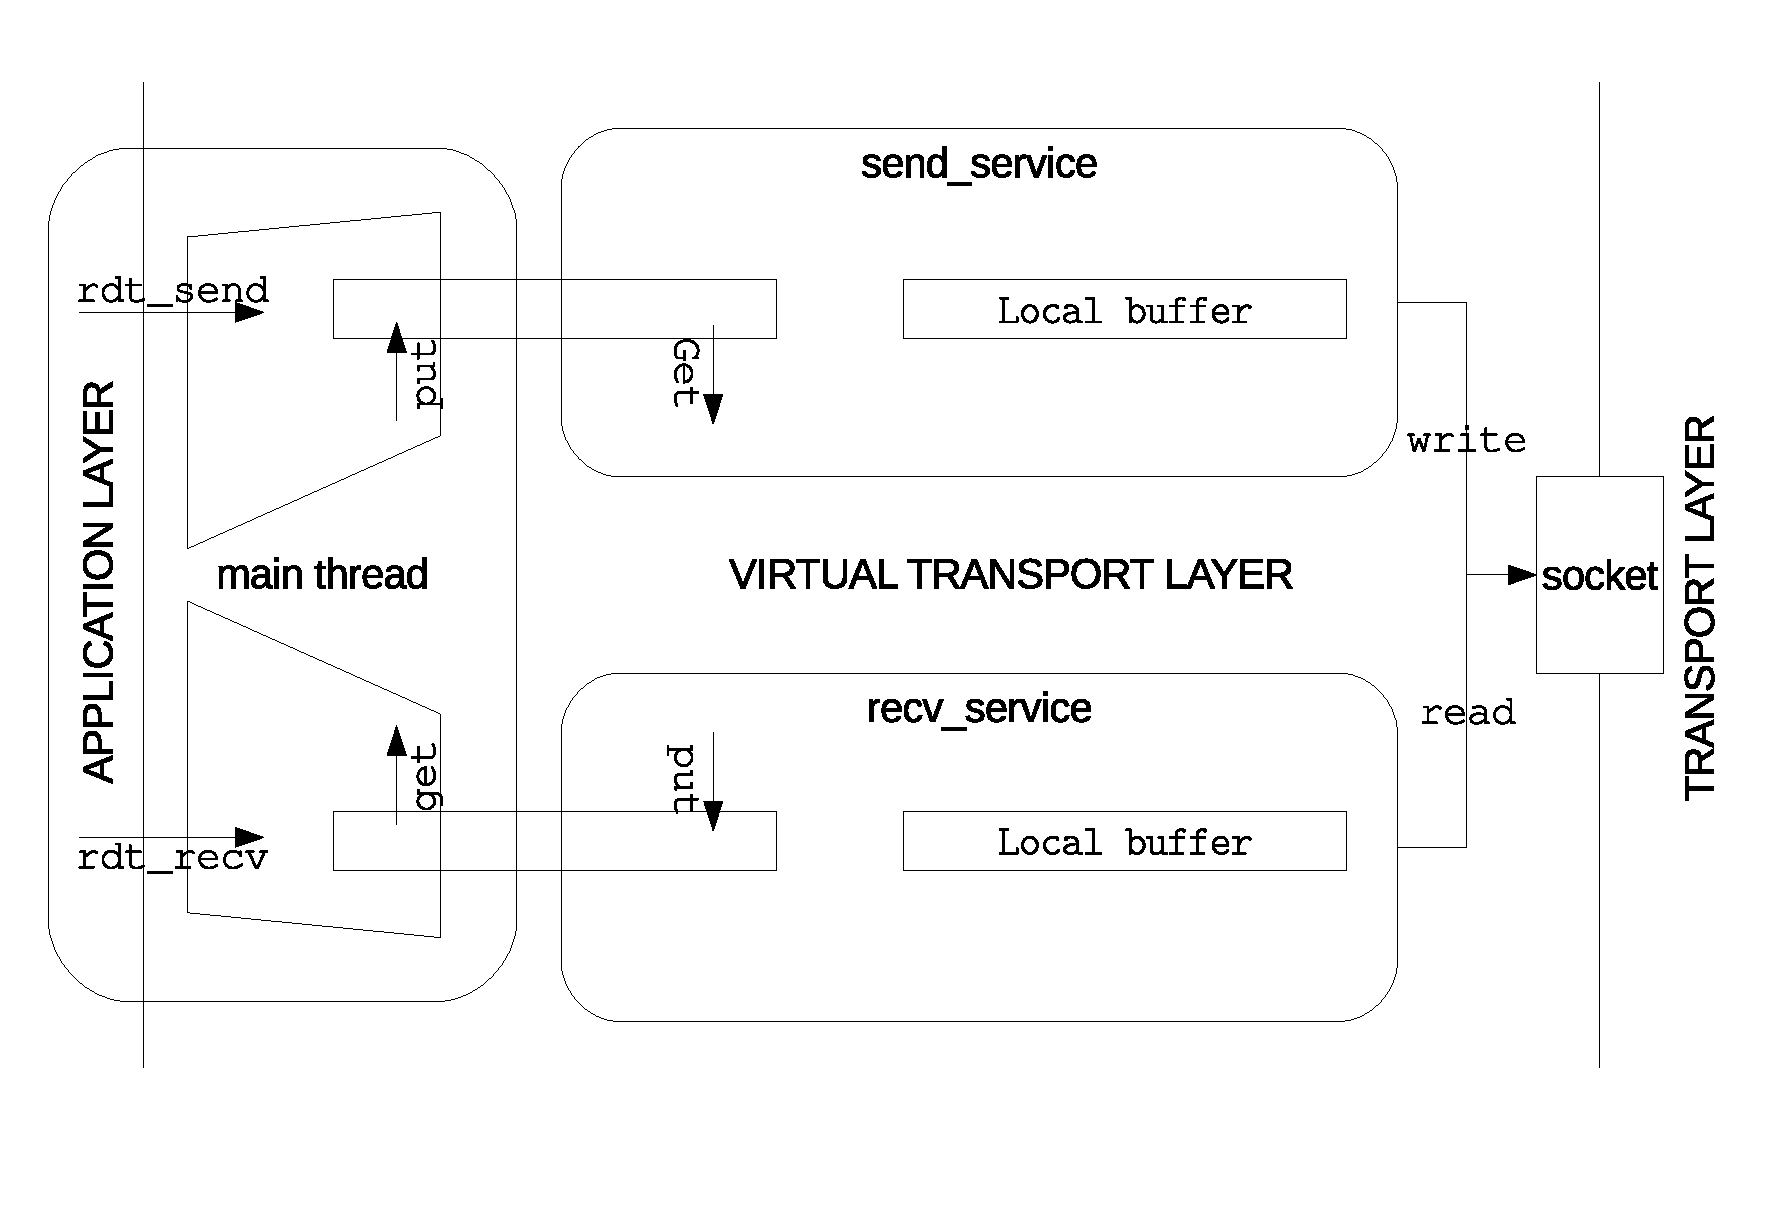
\includegraphics[scale=0.35]{images/structure_1}

Prima di passare a come viene implementato il \emph{selective repeat}, è 
necessario introdurre le strutture principale che ne supportano il 
funzionamento.\\
Come già detto, le unità di base con cui l'algoritmo ha a che fare sono
i segmenti che contengono i dati applicativi. Poiché tali segmenti sono
soggetti a ritrasmissioni, è necessario che vengano ``immagazzinati'' da 
qualche parte, inoltre, per quanto riguarda il lato destinatario, vanno
consegnati al livello applicativo in ordine, per queste ragioni, sia il 
servizio di invio che il servizio di ricezione sono dotati di buffer locali.\\
Tali buffer sono implementati tramite array di dimensione fissa e hanno una
capacità pari a MAXSEQNUM slot, in modo tale da far
corrispondere gli indici ai numeri di sequenza dei segmenti e 
garantirne un accesso immediato ($\mathcal{O}(1)$). Inoltre i buffer vengono
trattati come circolari, così da emulare naturalmente il riciclo dei numeri 
di sequenza.\\
Mentre il buffer del \emph{recv\_service} è implementato tramite un'array di 
strutture \emph{segment}, quello del \emph{send\_service} è un'array di 
strutture \emph{packet}, ovvero contenitori di segmenti e informazioni ad essi
relative necessarie al funzionamento del timeout, come istante di invio, quello
di scadenza ed un booleano che indica se il pacchetto è stato ritrasmesso.

\begin{lstlisting}[title=transport.h]
struct packet {
	struct segment sgt;
	struct timespec sendtime;
	struct timespec exptime;
	bool rtx;
};
\end{lstlisting}

Un'altra struttura fondamentale per l'algoritmo è la \emph{window}, che 
rappresenta le finestre di spedizione o ricezione delle due parti 
coinvolte.
\begin{lstlisting}[title=window.h]
struct window {
	unsigned int base;
	unsigned int width;
	struct bit_array ack_bar;	// 128 bit array
};
\end{lstlisting}
Tale struttura è composta da un'indice \emph{base} che rappresenta la base
della finestra, un intero \emph{width} che indica l'ampiezza massima della
finestra ed infine una struttura \emph{bit\_array} che non è altro che una
bitmask che tiene conto di quali segmenti sono arrivati a destinazione a 
partire dalla base della finestra.

[Disegno esempio bitmask] 

Infine, vi è la struttura necessaria alla gestione del timeout dei segmenti
inviati: una coda priotritaria i cui nodi sono puntatori
ai pacchetti presenti nel buffer locale di invio.\\
Ogni nodo è ordinato in base alla scadenza del timeout e una scansione 
periodica determina quali segmenti vanno ritrasmessi, appena si trova un 
segmento non scaduto non è necessario controllare i successivi
nella coda.
Questo meccanismo permette di gestire più timeot logici avendo un solo 
contatore hardware a disposizione.\\
In termini di prestazioni, avendo già N nodi nella coda, 
l'inserimento di un nuovo nodo richiede il confronto con tutti i
nodi che scadono prima, questo si effettua al più con un numero di passi
pari al numero di nodi presenti ($\mathcal{O}(N)$)
nel caso di timeout adattativo, invece se il timeout è costante non vi è bisogno
di alcun confronto poiché l'ultimo nodo inviato sarà l'ultimo a scadere e 
verrà semplicemente accodato (tempo $\mathcal{O}(1)$).
Per quanto riguarda l'estrazione del primo nodo da ritrasmettere, grazie 
all'inserimento prioritario, non è richiesta nessuna scansione, poiché il nodo 
in testa sarà il primo a scadere.\\
La coda è stata implementata in maniera tale da occupare meno memoria possibile,
infatti i nodi sono composti dagli indirizzi delle strutture \emph{packet}
presenti nel buffer locale, la coda tiene conto solo del loro ordinamento.

[disegno time\_queue]


\subsubsection{Mittente}
%
Il lato mittente del protocollo viene svolto principalmente dal 
\emph{send\_service} e in parte anche dal \emph{recv\_service}.\\
Quando il lato applicativo intende inviare un messaggio, richiama la funzione
\emph{rdt\_send} passando dati e relativa quantità in byte come argomenti.\\
La funzione controlla lo spazio disponibile sul buffer circolare condiviso
e immette un quantità di dati (in byte) possibilmente pari ad un multiplo di 
MSS, per consentire al servizio di invio di creare segmenti completamente pieni 
di dati significativi (size = MSS). Se non sono disponibili almeno MSS byte 
aspetta fintanto che non si libera lo spazio necessario. Naturalmente il 
processo viene ripetuto fintanto che non vengono passati tutti i dati 
applicativi.\\
Essendo, il buffer circolare, una risorsa condivisa tra thread principale e 
thread di invio, è stato necessario implementare dei meccanismi di 
sincronizzazione.\\
A tale scopo l'accesso esclusivo al buffer viene garantito da un mutex,
mentre, per quanto riguarda l'attesa per la disponibilità di spazio, il thread
principale attende su una variabile condizione che viene opportunamente segnalata
quando il servizio di invio svuota il buffer. A sua volta il thread principale
segnala la condizione al thread di invio che nel buffer sono presenti dati dopo
l'immissione degli stessi.
%
\begin{lstlisting}[title=trasport.h]
struct circular_buffer {
    pthread_mutex_t mtx;
    pthread_cond_t cnd_not_empty;
    pthread_cond_t cnd_not_full;
    unsigned int S;
    unsigned int E;
    char buf[CBUF_SIZE];
};
\end{lstlisting}
\begin{lstlisting}[title=trasport.c]
void rdt_send(const void *buf, size_t len)
{
    size_t free, tosend, left = len;

    while (left) {

        if (pthread_mutex_lock(&send_cb.mtx) != 0)
            handle_error("pthread_mutex_lock");

        /* check available space */
        while ((free =
                space_available(send_cb.S, send_cb.E, CBUF_SIZE))
				<= MSS)
            if (pthread_cond_wait(&send_cb.cnd_not_full, 
				&send_cb.mtx) != 0)
                handle_error("pthread_cond_wait");

        /* calculate how much data to send */
        tosend =  free > left ?	left : free / MSS * MSS;

        memcpy_tocb(send_cb.buf, buf + len - left, tosend, 
					send_cb.E, CBUF_SIZE);

        send_cb.E = (send_cb.E + tosend) % CBUF_SIZE;

        if (pthread_mutex_unlock(&send_cb.mtx) != 0)
            handle_error("pthread_mutex_unlock");

        if (cond_event_signal(&e, PKT_EVENT) == -1)
            handle_error("cond_event_signal()");

        left -= tosend;
    }
}
\end{lstlisting}
%
Segnalata la presenza di dati sul buffer condiviso, il servizio di invio,
appena può, richiama la funzioni \emph{empty\_buffer} e \emph{send\_packets}.
%
\begin{lstlisting}[title=transport.c]
	.....

switch (e->type) {

case PKT_EVENT:

	/* empty shared buffer and put segments into the local one */
	empty_buffer(cb, pkts_buffer, &w, &lastseqnum);
	/* send available segments */
	send_packets(sockfd, loss, pkts_buffer, lastseqnum, &w,
				 &time_queue, &timeout);

	break;

case ACK_EVENT:
    // ack work .....
	break;

default:
	fputs("Unexpected event type\n", stderr);
	break;
}
	.....

\end{lstlisting}
%
La funzione \emph{empty\_buffer} ha il compito di svuotare il buffer condiviso,
creare i segmenti ed immagazzinarli nel buffer locale, in cui vi rimarranno
(saranno validi) fino a quando non sarà tornato indietro l'ack relativo e 
tutti quelli dei segmenti con numero di sequenza precedente.
%
\begin{lstlisting}[title=transport.c]
void empty_buffer(struct circular_buffer *cb, struct packet *pkts,
                  struct window *w, unsigned int *last_seqnum)
{
    size_t data, size;

    if (pthread_mutex_lock(&cb->mtx) != 0)
        handle_error("pthread_mutex_lock");

    while (cb->S != cb->E && 
           cbuf_free(w->base, *last_seqnum, MAXSEQNUM)) {
        // shared buffer not empty and local buffer has free slots

        data = data_available(cb->S, cb->E, CBUF_SIZE);
        size = data < MSS ? data : MSS;

        /* store a new packet */
        store_pkt(pkts, *last_seqnum, size, cb);
        *last_seqnum = (*last_seqnum + 1) % MAXSEQNUM;
        cb->S = (cb->S + size) % CBUF_SIZE;

        if (pthread_cond_signal(&cb->cnd_not_full) != 0)
            handle_error("pthread_cond_signal");
    }

    if (pthread_mutex_unlock(&cb->mtx) != 0)
        handle_error("pthread_mutex_unlock");
}
\end{lstlisting}
%
La funzione, fintanto che sono presenti dati sul buffer condiviso e ci sono 
slot liberi in quello locale, estrae al più MSS byte per poi creare un segmento,
che verrà posizionato in uno slot del buffer locale tramite la 
funzione \emph{store\_pkt}.\\
Ogni volta che un segmento viene estratto ed inserito nel buffer locale, viene anche 
aggiornato l'indice \emph{last\_seqnum} che indica il numero di sequenza del
prossimo pacchetto che verrà immagazzinato e quindi corrisponde al primo slot
libero del buffer locale.
%
\begin{lstlisting}[title=transport.c]
void store_pkt(struct packet *base, uint8_t seqnum, size_t size,
               struct circular_buffer *cb)
{
    struct packet *pkt = base + seqnum;
    struct segment *sgt = &(pkt->sgt);

    sgt->seqnum = seqnum;
    sgt->size = size;
    memcpy_fromcb(sgt->payload, cb->buf, size, cb->S, CBUF_SIZE);

    pkt->rtx = false;
}
\end{lstlisting}
%
La funzione \emph{send\_packets} si occupa di inviare i segmenti presenti nel
buffer locale fino a che l'indice nextseqnum non supera il limite stabilito
dall'ampiezza della finestra di invio.
%
\begin{lstlisting}[title=transport.c]
void send_packets(int sockfd, double loss, struct packet *pkts,
                  unsigned int lastseqnum, struct window *w,
                  struct queue_t *time_queue, 
				  struct timespec *timeout)
{
    static unsigned int nextseqnum = 0;
    struct packet *pkt;         // packet pointer

    while (in_window(w, nextseqnum) &&
           more_packets(nextseqnum, w->base, lastseqnum)) {
        // nextseqnum is inside the window and
        // there are packets not sent yet

        pkt = pkts + nextseqnum;
        send_packet(sockfd, pkt, loss);

        /* set packet sendtime and exptime */
        pkt_settime(pkt, timeout);

        prio_enqueue(pkt, time_queue, pkt_exptimecmp);
        nextseqnum = (nextseqnum + 1) % MAXSEQNUM;
    }
}
\end{lstlisting}
%
Quando un segmento viene inviato vengono registrati il tempo di invio e di
scadenza, inoltre un riferimento al pacchetto viene inserito nella coda 
per la gestione del timeout.\\
Una volta che almeno un segmento è stato inviato, entra in gioco il 
\emph{recv\_service} che, bloccato in lettura sulla socket, attende l'arrivo
degli ack.
Quando ne giunge uno, appena possibile, lo segnala al \emph{send\_service} 
inserendo il numero di sequenza nella variabile \emph{acknum} della
struttura condivisa \emph{event}.
%
\begin{lstlisting}[title=transport.c]
.....

for (;;) {

	r = read(sockfd, buffer, max_recvsize);

	.....

	/* segment received */
	if (r == sizeof(struct segment)) {
		// segment work .....
		continue;
	}

	/* ACK received */
	if (r == sizeof(acknum)) {
		acknum = (uint8_t) * buffer;
		if (cond_ack_event_signal(e, acknum) == -1)
			handle_error("cond_event_signal()");
		continue;
	}

.....
\end{lstlisting}
%
Alla ricezione del segnale di ack il servizio di invio rimuove il nodo 
corrispondente al numero di sequenza dell'ack, aggiorna il valore 
del timeout e aggiorna la finestra, eventualmente facendola scorrere 
se il numero di sequenza è relativo alla base della finestra.
%
\begin{lstlisting}[title=transport.c]
switch (e->type) {

    case PKT_EVENT:
        // pkt work .....
        break;

    case ACK_EVENT:
        acknum = e->acknum;
        if (params->adaptive)
            update_timeout(&timeout, pkts_buffer + acknum);
		remove_pkt_timeout(&time_queue, acknum);
        update_window(&w, acknum);
        empty_buffer(cb, pkts_buffer, &w, &lastseqnum);
        send_packets(sockfd, loss, pkts_buffer, lastseqnum, &w,
                     &time_queue, &timeout);
        break;

    default:
        fputs("Unexpected event type\n", stderr);
        break;
    }
}
\end{lstlisting}
Il valore del timeout viene aggiornato soltanto quando arrivano ack relativi
a segmenti che non hanno subito ritrasmissioni.\\
La funzione \emph{adapt\_timeout} aggiorna il timeout in base a quanto tempo
è trascorso dall'invio del segmento fino alla ricezione dell'ack, come
descritto nel libro di testo \cite{kurose}, secondo la formula [formula].
%
%	FORMULA
%
Il tempo trascorso è calcolato sottraendo all'istante corrente quello di invio
del segmento ricevuto, questo risulterà leggermente maggiore, perché
non viene calcolato nel momento esatto in cui arriva effettivamente l'ack.
%
\begin{lstlisting}[title=transport.c]
void update_timeout(struct timespec *timeout, struct packet *pkt)
{
    struct timespec now, elapsed;

    /* check if packet was retransmitted */
    if (pkt->rtx)
        return;

    if (clock_gettime(CLOCK_REALTIME, &now) == -1)
        handle_error("ack timestamp");

    if (timespec_sub(&elapsed, &now, &pkt->sendtime) == -1)
        handle_error("calculating elapsed time");

    adapt_timeout(timeout, &elapsed);
}
\end{lstlisting}
L'aggiornamento della finestra consiste nel contrassegnare il segmento come
ricevuto. Questo viene fatto impostando il relativo bit a 1 nella barra degli
ack della finestra.\\
Se il numero di sequenza corrisponde alla base della finestra, il bit non viene
impostato e viene fatta scorrere la finestra relativamente al prossimo segmento
per cui deve ancora arrivare un riscontro.
\begin{lstlisting}[title=window.c]
void update_window(struct window *w, uint8_t acknum)
{
    unsigned int i, s;

    if (acknum == w->base) {
        /* shift ack bar to the first unmarked bit */
        s = calc_shift(w);
        if (shift(&w->ack_bar, s) == -1)
            handle_error("shift()");
        /* slide window */
        w->base = (w->base + s) % MAXSEQNUM;
    }
    else if (in_window(w, acknum)) {
        /* calculate distance from window's base */
        i = distance(w, acknum);
        /* mark packet as acked */
        if (set_bit(&w->ack_bar, i) == -1)
            handle_error("set_bit()");
    }
}
\end{lstlisting}
Infine, se c'è stato uno scorrimento della finestra di invio, si libererà
dello spazio sul buffer circolare e sarà possibile 
inviare i segmenti successivi, pertanto vengono richiamate le funzioni
\emph{empty\_buffer} e \emph{send\_packets} già descritte in precedenza.\\
%
L'ultimo evento a cui il mittente deve reagire riguarda la scadenza del 
timeout di un segmento.\\
Ciò avviene quando la \emph{pthread\_cond\_timedwait} restituisce la 
costante ETIMEDOUT come valore di ritorno, in tal caso viene chiamata
la funzione \emph{resend\_expired} che determina quali pacchetti sono 
scaduti e li ritrasmette.
\begin{lstlisting}[title=window.c]
for (;;) {

    .....

	condret = 0;
	while (e->type == NO_EVENT && condret != ETIMEDOUT) {
		// no events and timeout not expired

		/* calculate remaining time to wait */
		if (calc_wait_time(&time_queue, &wait_time) == -1) {
			/* timeout expired: resend expired packets */
			resend_expired(sockfd, loss, &time_queue, &timeout, &w);
			continue;
		}

		condret = pthread_cond_timedwait(&e->cnd_event, &e->mtx,
                                         &wait_time);
		if (condret != 0 && condret != ETIMEDOUT)
			handle_error("pthread_cond_timedwait");
	}


	/* TIMEOUT EVENT */
	if (condret == ETIMEDOUT) {
		resend_expired(sockfd, loss, &time_queue, &timeout, &w);
		continue;
	}

    .....
}
\end{lstlisting}
La funzione per la ritrasmissione estrae segmenti fintanto
che non ne trova uno che non sia scaduto, ognuno di essi viene ritrasmesso,
marcato come tale, e vengono aggiornati i tempi di invio e di
scadenza, infine viene di reinserito nella coda del timeout.
\begin{lstlisting}[title=transport.c]
void resend_expired(int sockfd, double loss, 
                    struct queue_t *time_queue,
                    struct timespec *timeout, struct window *w)
{
    struct packet *pkt;

    while (time_queue->head != NULL) {

        /* fetch first to expire packet */
        pkt = get_head_packet(time_queue);

        if (!pkt_expired(pkt))
            break;

        dequeue(time_queue);

        send_packet(sockfd, pkt, loss);
        pkt->rtx = true;

        /* set packet time */
        pkt_settime(pkt, timeout);

        prio_enqueue(pkt, time_queue, pkt_exptimecmp);
    }
}
\end{lstlisting}
La funzione \emph{pthread\_cond\_timedwait} attende il verificarsi degli 
eventi di ricezione di dati dal livello superiore, oppure di ricezione di
un ack, per un tempo calcolato ad ogni ciclo tramite la funzione
\emph{calc\_wait\_time}, che imposta il tempo di attesa in base a quanto 
ne rimane alla scadenza del timeout del primo segmento.\\
Se la coda non contiene nodi, il timeout viene impostato ad un valore
abbastanza elevato per fare in modo che il thread non venga svegliato 
inutilmente, è sufficiente impostarlo nell'ordine delle decine di secondi.
\begin{lstlisting}[title=transport.c]
int calc_wait_time(struct queue_t *q, struct timespec *wait_time)
{
    struct packet *pkt;
    struct timespec now, left;

    if (clock_gettime(CLOCK_REALTIME, &now) == -1)
        handle_error("clock_gettime()");

    if (!q->head) {
        /* queue is empty: turn off the timeout */
        left.tv_sec = 30;
        left.tv_nsec = 0;
    } else {
        pkt = get_head_packet(q);

        /* calculate remaining time to timeout */
        if (timespec_sub(&left, &pkt->exptime, &now) == -1)
            /* now > exptime: timeout expired */
            return -1;
    }

    timespec_add(wait_time, &now, &left);
    return 0;
}
\end{lstlisting}

\subsubsection{Selective Repeat: ricevente}
Il lato mittente del protocollo viene svolto soltanto dal 
\emph{recv\_service}, che si occupa di gestire il riordino
e la consegna a livello applicativo dei segmenti che giungono 
dalla rete, ed eventualmente di inviare i riscontri al mittente.
\begin{lstlisting}[title=transport.c]
void *recv_service(void *p)
{
    .....

    for (;;) {

        r = read(sockfd, buffer, max_recvsize);

        if (r == -1) {
            // error ot timeout .....     
        }

        /* segment received */
        if (r == sizeof(struct segment)) {

            sgt = (struct segment *) buffer;
            if (process_segment(
                sgt, segments_cb, &recv_window, cb)) {
                /* send ACK */
                if (udt_send
                    (tools->sockfd, &sgt->seqnum, sizeof(uint8_t),
                     loss) == -1)
                    handle_error("udt_send() - sending ACK");
            }
            continue;
        }

        /* ACK received */
        if (r == sizeof(acknum)) {
            // ACK work .....
            continue;
        }
    }
    .....
}
\end{lstlisting}
Il thread, bloccato in lettura sulla socket, quando riceve un segmento
chiama la funzione \emph{process\_segment} che controlla il numero di 
sequenza. Se questo cade all'interno della finestra, si controlla se non
è un duplicato ed in tal caso il segmento viene salvato nel buffer locale
e viene marcato come ``giunto'' impostando ad 1 il bit relativo nella finestra,
poi, se coincide con la base della finestra, vengono consegnati a livello 
applicativo tutti i segmenti
consecutivi presenti nel buffer a partire dalla base, infine la funzione
restituisce \emph{true} per segnalare che il segmento è valido ed 
è necessario inviare l'ack al mittente.\\
Se il numero di sequenza cade nell'intervallo precedente alla base della
finestra \emph{[base - ampiezza; base - 1]},
il segmento è già stato ricevuto e quindi 
viene ignorato, ma la funzione restituisce comunque il valore \emph{true}
poiché è necessario inviare l'ack.\\
In tutti gli altri casi, un eventuale segmento viene ignorato e la funzione 
restituisce false per non far inviare il relativo ack al mittente.
\begin{lstlisting}[title=transport.c]
bool process_segment(struct segment *sgt, 
                     struct segment *segments_cb,
                     struct window *w, struct circular_buffer *cb)
{
    static unsigned int S = 0;
    unsigned int i, s, seqnum;

    seqnum = sgt->seqnum;
    fprintf(stderr, "received segment %u\n", seqnum);

    if (in_window(w, seqnum)) {

        /* calculate seqnum distance from the base of the window */
        i = distance(w, seqnum);

        /* check if the segment is a duplicate */
        if (is_duplicate(w, i)) {
            //fputs("Already received\n", stderr);
            return true;
        }

        /* store the segment */
        segments_cb[(S + i) % w->width] = *sgt;

        /* mark segment as arrived */
        if (set_bit(&w->ack_bar, i) == -1)
            handle_error("set_bit()");
        fprint_window(stderr, w);

        if (seqnum == w->base) {
            /* calculate the number of consecutive segments */
            s = calc_shift(w);
            /* deliver consecutive segments */
            for (i = 0; i < s; i++) {
                deliver_segment(cb, segments_cb + S);
                S = (S + 1) % w->width;
            }
            /* update window indexes */
            shift_window(w, s);
            w->base = (w->base + s) % MAXSEQNUM;
        }
        return true;
    } else if (in_prewindow(w, seqnum)) {
        //fputs("Already received\n", stderr);
        return true;
    }
    return false;
}
\end{lstlisting}
Nel caso in cui il numero di sequenza coincide con la base della finestra,
vengono contati i bit consecutivi impostati ad 1 e, successivamente, 
vengono consegnati a livello applicativo altrettanti segmenti (a partire 
da quello appena arrivato) tramite la funzione \emph{deliver\_segment}, 
che ne immette il payload nel buffer circolare condiviso appena c'è spazio
disponibile.
\begin{lstlisting}[title=transport.c]
void deliver_segment(struct circular_buffer *cb, 
                     struct segment *sgt)
{
    if (pthread_mutex_lock(&cb->mtx) != 0)
        handle_error("pthread_mutex_lock");

    /* check free space */
    while (space_available(cb->S, cb->E, CBUF_SIZE) <= MSS) 
        if (pthread_cond_wait(&cb->cnd_not_full, &cb->mtx) != 0)
            handle_error("pthread_cond_wait");

    memcpy_tocb(cb->buf, sgt->payload, sgt->size, cb->E, 
                CBUF_SIZE);
    cb->E = (cb->E + sgt->size) % CBUF_SIZE;

    if (pthread_cond_signal(&cb->cnd_not_empty) != 0)
        handle_error("pthread_cond_signal");
    if (pthread_mutex_unlock(&cb->mtx) != 0)
        handle_error("pthread_mutex_unlock");
}
\end{lstlisting}

